
\chapter{考虑粗糙壁面的转捩预测方法}
根据第二章中对$SST~\gamma-\overline{Re_\theta}$转捩模型的介绍和实际算例计算,说明了使用该模型计算转捩时能较好的模拟bypass转捩
 
\section{表面粗糙度模型介绍}
\subsection{粗糙增长因子$A_r$输运方程}
\subsection{边界条件修正}
\subsection{耦合转捩模型}

\section{粗糙转捩模型算例验证}
本节通过对分离零压力梯度粗糙平板,顺、逆压力梯度粗糙平板,粗糙NACA0012翼型和粗糙S814翼型这三个算例中表面粗糙度对转捩的影响进行分析,进而对耦合$A_r$输运方程的$SST~\gamma-\overline{Re_\theta}$粗糙转捩模型的预测水平进行检验。
\subsection{粗糙平板算例}
本小节选用Fenindt的粗糙平板实验 \ucite{feindt1957untersuchungen}作为验证算例,该实验最早被Dassler等人\ucite{dassler2010modelling}用来进行模型的验证。Feindt\ucite{feindt1957untersuchungen}设置了不同压力梯度来研究粗糙高度和转捩位置的关系。在使用粗糙转捩模型进行数值模拟时,保持入口高度$h_0$和平板长度$L$固定,除了零压力梯度算例外,顺、逆压力梯度算例通过设置上壁面的形状来形成收缩-扩张管道来实现。非零压力梯度的上表面轮廓通过函数$h(x)$确定:
\begin{equation} \label{roughnessupper}
h(x)=\frac{{h_0}^2}{\sqrt{1.0-PG}}
\end{equation}
在该表达式中,参数$PG$设置为于Feindt\ucite{feindt1957untersuchungen}实验中两个非零压力梯度测试的条件相匹配。入口高度$h_0$设置为$0.1495L$,以匹配Dassler等人的原始CFD算例中的网格。由Dassler等人\ucite{dassler2010modelling}模拟的压力梯度可知压力梯度参数$PG$设置如下:
\begin{equation}
PG = \left\{ \begin{array}{rcl}
0.458x& \mbox{逆压梯度}
\\-0.430x & \mbox{顺压梯度}
\end{array}\right.
\label{PG参数设置}
\end{equation}
式中$x$为平板流向距离,平板长度$L$设置为1m,根据根据公式\autoref{roughnessupper}和 \ref{PG参数设置},可以得到粗糙平板计算域的上边界轮廓,网格分布如图3-1、3-2和3-3所示。三套网格在边界层上第一层无量纲化网格高度$y^+$均小于1。
\begin{figure}[htbp]
	\centering
	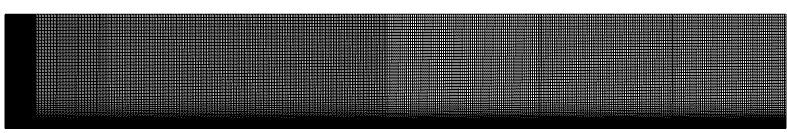
\includegraphics[scale=1]{figures/zero_mesh.jpg}
	\caption{无压力梯度平板}
\end{figure}
\begin{figure}[htbp]
	\centering
	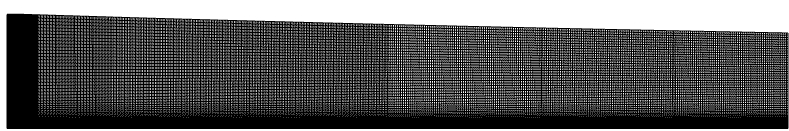
\includegraphics[scale=1]{figures/favorable_mesh.png}
	\caption{顺压力梯度平板}
\end{figure}
\begin{figure}[htbp]
	\centering
	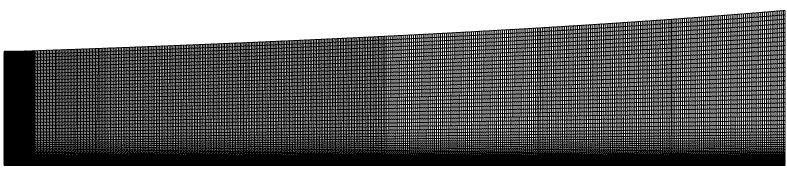
\includegraphics[scale=1]{figures/adverse_mesh.png}
	\caption{逆压力梯度平板}
\end{figure}
在计算边界条件设置上,入口马赫数为0.2。自由来流湍流度为$1.0\%$,基于平板长度的雷诺数设置为$1.3\times10^6$。根据以上设置对从$0\mu m$到$257\mu m$的八个不同粗糙高度的平板进行计算,对于不考虑粗糙度影响的壁面$k_s=0\mu m$具体的边界条件设置如表3-1所示。
\begin{table}[htbp]
	\centering
	\caption{粗糙平板计算条件}
	\label{tab:my_label}
	\begin{tabular}{|>{\centering\arraybackslash}p{1.5cm}|>{\centering\arraybackslash}p{1.5cm}|>{\centering\arraybackslash}p{1.5cm}|>{\centering\arraybackslash}p{5cm}|} % 每列的宽度可以根据需要进行调整
		\hline
		$M_a$ & $R_e$ & $T_u\%$ &  $k_s(\mu m)$ \\ \hline
		0.2 & $1.3\times10^6$ & 1.5 & 0,40,120,193,220,275  \\ \hline
	\end{tabular}
\end{table}

为了观察粗糙度对平板边界层转捩的影响,由于表面表面摩擦力系数$C_f$能直观地反映出转捩位置,应当从$C_f$入手观察。如图3-4所示,该图展示了表面摩擦系数$C_f$受粗糙高度的影响,可以清晰地看出随着$k_s$的增加,无压力梯度粗糙平板上的转捩位置不断提前。


\subsection{粗糙NACA0012翼型}
\subsection{粗糙S814翼型}





\section{本章小结}


\clearpage
\endinput
